\chapter{RL Foundations for Language Models}
\label{ch:rl-foundations}
\raggedbottom

In January 2025, DeepSeek released R1~\cite{deepseekai2025r1}, a reasoning model family whose most striking result came from an intermediate model called R1-Zero. Starting from a pretrained base model, R1-Zero learned to produce long chains of thought, self-correct mid-solution, and backtrack when stuck without a human-written reasoning-trace dataset. The training signal was sparse and verifiable: did the final math answer match the ground truth? The algorithm was reinforcement learning. No learned reward model was needed for that stage. A verifiable reward and a policy-gradient-style update were enough to surface reasoning behaviors that, a few months earlier, had mostly been visible in proprietary systems.

Chapter~\ref{ch:preference-learning} taught you to optimize a language model for preferences without RL machinery. DPO collapses the reward-model--plus--PPO pipeline into a single supervised loss---elegant, stable, and sufficient for many alignment tasks. But \S\ref{sec:dpo-limits} was honest about the boundary: DPO sharpens existing behavior; it does not create new capabilities. When the goal is to push the model beyond what any demonstration or preference pair can teach---sustained multi-step reasoning, novel problem-solving strategies, self-correction---you need a training signal that evaluates \emph{outcomes}, not just comparisons. That signal is a reward function, and the framework for optimizing it is reinforcement learning.

Think of the difference like learning to cook. SFT is following a recipe step by step. DPO is tasting two dishes and learning which one the diner preferred. RL is cooking freely, getting a score from a food critic, and adjusting your technique based on nothing but that score. The score says \emph{how good} the dish was, not \emph{how to make it better}---you have to figure out the ``how'' yourself. This chapter teaches the machinery for that process.

It is not a comprehensive RL course. It is an LLM-tailored crash course that develops the machinery Chapters~\ref{ch:rlhf} and~\ref{ch:reasoning-rl} rely on most heavily: MDPs, policy gradients, variance reduction, PPO-style updates, and KL regularization. By the end, you will have the vocabulary to read modern RLHF and reasoning-RL papers, and you will understand why autoregressive text generation removes many of the complications that make classical RL difficult.

\paragraph{What this chapter covers.} Three ideas organize the chapter:

\begin{enumerate}[nosep]
  \item \textbf{The formalism.} What is an MDP, and why does LLM generation collapse it into a surprisingly simple special case? (\S\ref{sec:why-rl}--\S\ref{sec:llm-mdp})
  \item \textbf{The algorithms.} How do you compute a gradient through a reward signal? REINFORCE, importance sampling, and PPO-style clipped updates---the core family behind RLHF and the foundation for many reasoning-RL variants. (\S\ref{sec:policy-gradient}--\S\ref{sec:ppo})
  \item \textbf{The constraint.} Why does LLM RL specifically need a KL penalty to the reference policy, and what goes wrong without it? (\S\ref{sec:kl-rl})
\end{enumerate}

\paragraph{Running example.} Your 3B model from Project~3 has been instruction-tuned (Chapter~\ref{ch:instruction-tuning}) and preference-aligned with DPO (Chapter~\ref{ch:preference-learning}). Suppose you now want it to solve grade-school math problems---not by imitating solution traces, but by discovering effective reasoning strategies on its own. You have a verifier that checks final answers. How do you turn that binary signal into a gradient update? Every concept in this chapter will be instantiated on this setup.


\subsection*{Learning Objectives}

After completing this chapter, you should be able to:

\begin{enumerate}
  \item Define the components of a Markov Decision Process (state, action, reward, policy, value) and write the Bellman equation.
  \item Explain why autoregressive language generation is a degenerate MDP with deterministic transitions and sparse reward.
  \item Derive the REINFORCE gradient estimator and explain why it has high variance.
  \item Explain why PPO uses a clipped surrogate objective instead of the raw policy gradient.
  \item Articulate why LLM RL requires a KL constraint to a reference policy, and connect this to the KL-constrained objective from Chapter~\ref{ch:preference-learning}.
\end{enumerate}


\subsection*{Notation}

\begin{center}
\begin{tabular}{ll}
\toprule
Symbol & Meaning \\
\midrule
$s$ & State in the MDP \\
$a$ & Action \\
$r(s, a)$ & Reward function \\
$\pi_\theta(a \mid s)$ & Policy (parameterized by $\theta$) \\
$V^\pi(s)$ & Value function: expected return from state $s$ under $\pi$ \\
$A^\pi(s, a)$ & Advantage function: $Q^\pi(s,a) - V^\pi(s)$ \\
$\gamma$ & Discount factor \\
$\tau$ & Trajectory (sequence of states and actions) \\
$R(\tau)$ & Total return for trajectory $\tau$ \\
$\hat{A}_t$ & Estimated advantage at time step $t$ \\
$\epsilon$ & PPO clipping parameter \\
$\beta$ & KL penalty coefficient \\
$\pi_{\text{ref}}$ & Reference policy (frozen SFT checkpoint) \\
\bottomrule
\end{tabular}
\end{center}


\subsection*{Timeline of Key Contributions}

\begin{center}
\begin{tabularx}{\textwidth}{@{}lX@{}}
\toprule
\textbf{Year} & \textbf{Contribution} \\
\midrule
1992 & Williams publishes REINFORCE: the first general-purpose policy gradient algorithm \\
1999 & Sutton et al.\ formalize the policy gradient theorem \\
2015 & Schulman et al.\ introduce TRPO: trust-region optimization for policy gradients \\
2016 & Schulman et al.\ introduce GAE: a practical method for advantage estimation \\
2017 & Schulman et al.\ publish PPO: a simpler alternative to TRPO that uses clipping instead of constraints \\
2017 & Christiano et al.\ apply RL from human preferences to Atari and MuJoCo; establish the RLHF paradigm \\
2022 & Ouyang et al.\ (InstructGPT) instantiate PPO on language model trajectories at production scale \\
2025 & DeepSeek-R1-Zero demonstrates large-scale reasoning RL with GRPO-style critic-free policy optimization and verifiable rewards \\
\bottomrule
\end{tabularx}
\end{center}


%----------------------------------------------------------------------
\section{What RL Is and Why Language Models Use It}
\label{sec:why-rl}

Supervised learning requires a target. In pretraining, the target is the next token. In SFT (Chapter~\ref{ch:instruction-tuning}), the target is a human-written response. In DPO (Chapter~\ref{ch:preference-learning}), the target is implicit---a pairwise preference between two responses. In every case, the training signal says \emph{what} the model should produce.

Reinforcement learning does something different. It gives the model a \emph{reward signal}---a scalar score for each complete output---and asks it to figure out how to produce high-scoring outputs on its own. There is no demonstration to imitate, no pair to compare. The model generates a response, receives a score, and adjusts its parameters to make high-scoring responses more likely and low-scoring responses less likely.

\subsection{When SFT and DPO Are Not Enough}

Three situations where you need the reward-and-optimize loop:

\paragraph{The capability is hard to specify by demonstration.} Humans can write reasoning traces, but they cannot easily enumerate every useful self-correction, backtracking move, or search strategy a model might discover. Writing a single chain-of-thought solution to a math problem teaches the model to imitate \emph{that} solution. Verifiable RL can reward the outcome while leaving the path open---and the model may discover strategies no human demonstrated.

\paragraph{The evaluation is objective but the path is creative.} Given a coding problem with unit tests, there are many valid solutions. SFT on one solution teaches imitation of that solution. RL with test-pass reward encourages the model to find \emph{any} solution that passes---including ones no human wrote. The same logic applies to mathematical proof, constrained generation, and optimization problems.

\paragraph{Preference data cannot capture the signal.} DPO requires preference pairs. For safety alignment at frontier scale, the signal may need to be denser, more structured, or more adaptive than static preference datasets allow. RLHF (Chapter~\ref{ch:rlhf}) uses a learned reward model that can score any response on the fly, adapting to the current policy's behavior rather than relying on a fixed dataset.

\begin{figure}[t]
\centering
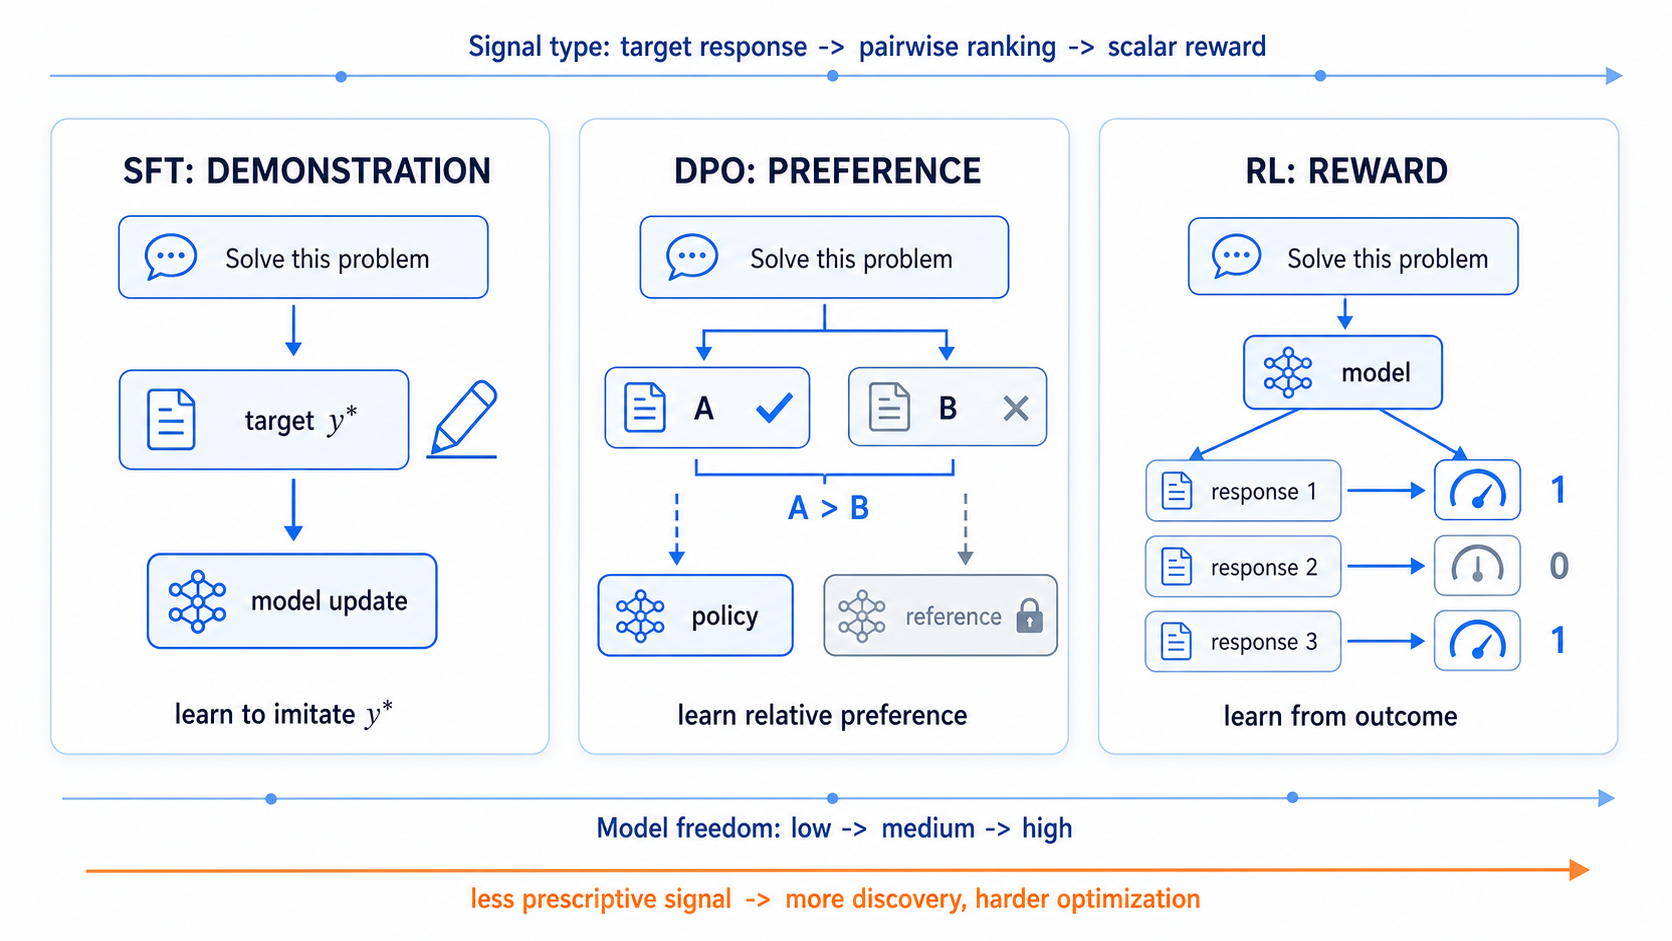
\includegraphics[width=0.95\textwidth]{figures/ch14/fig_signal_comparison.png}
\caption{\textbf{Three training paradigms, three signal types.} SFT uses demonstrations (complete target responses). DPO uses preferences (pairwise comparisons). RL uses reward signals (scalar scores for complete outputs). Each paradigm provides a progressively less constrained signal: demonstrations prescribe the output, preferences rank outputs, rewards evaluate outcomes. The less constrained the signal, the more room the model has to discover its own strategies---but the harder the optimization becomes.}
\label{fig:signal-comparison}
\end{figure}

\paragraph{The core trade-off.} Demonstrations are easy to learn from but constrain the model to imitate. Rewards are harder to learn from but allow the model to discover. RL is the machinery for converting reward signals into parameter updates. The rest of this chapter develops that machinery.

\begin{quickrecap}
\textbf{Quick Recap.}
\begin{itemize}[nosep,leftmargin=1.5em]
  \item SFT learns from demonstrations, DPO learns from preferences, RL learns from reward signals.
  \item RL is needed when the desired behavior cannot be demonstrated, when evaluation is objective but solutions are creative, or when preference data is insufficient.
  \item The trade-off: weaker supervision gives the model more freedom but makes optimization harder.
\end{itemize}
\textit{Next: the formal framework that makes ``learning from reward'' precise.}
\end{quickrecap}


%----------------------------------------------------------------------
\section{MDP Formalism}
\label{sec:mdp}

Reinforcement learning formalizes sequential decision-making as a \textbf{Markov Decision Process (MDP)}. An MDP is defined by five components. We state each one generally and immediately ground it in language generation:

\begin{enumerate}[nosep]
  \item \textbf{State space $\mathcal{S}$}: the set of all situations the agent can be in. For a language model, the state at step $t$ is the prompt plus all tokens generated so far: $s_t = (x, y_1, \ldots, y_{t-1})$.
  \item \textbf{Action space $\mathcal{A}$}: the set of all actions available. For a language model, this is the vocabulary $\mathcal{V}$---each action is choosing the next token.
  \item \textbf{Transition function $P(s' \mid s, a)$}: the probability of reaching state $s'$ after taking action $a$ in state $s$. For text generation, this is deterministic: appending token $a_t$ to $s_t$ always gives $s_{t+1} = s_t \oplus a_t$. No dice rolls, no physics noise.
  \item \textbf{Reward function $r(s, a)$}: the scalar feedback after taking action $a$ in state $s$. In LLM RL, reward is typically zero at every step except the last, where a verifier or reward model scores the complete response.
  \item \textbf{Discount factor $\gamma \in [0, 1)$}: how much the agent values future rewards relative to immediate ones. In LLM RL, $\gamma$ is usually set to 1 (no discounting) because episodes are short and all reward arrives at the end.
\end{enumerate}

Notice how many simplifications appeared before we even started: deterministic transitions, sparse reward, no discounting. Section~\ref{sec:llm-mdp} will unpack these in full. For now, we continue with the general formalism to define the quantities that every RL algorithm uses.

A \textbf{policy} $\pi(a \mid s)$ is a probability distribution over actions given the current state---for your 3B model, this is simply the next-token distribution $\pi_\theta(y_t \mid x, y_{<t})$. The agent's goal is to find a policy that maximizes the expected \textbf{return}---the discounted sum of future rewards:

\begin{equation}
\label{eq:return}
R(\tau) = \sum_{t=0}^{T} \gamma^t \, r(s_t, a_t)
\end{equation}

where $\tau = (s_0, a_0, s_1, a_1, \ldots, s_T, a_T)$ is a trajectory.

\subsection{The Value Function and Bellman Equation}

The \textbf{value function} $V^\pi(s)$ is the expected return starting from state $s$ and following policy $\pi$:

\begin{equation}
\label{eq:value}
V^\pi(s) = \mathbb{E}_\pi\!\left[\sum_{t=0}^{T} \gamma^t \, r(s_t, a_t) \;\middle|\; s_0 = s\right]
\end{equation}

The value function satisfies the \textbf{Bellman equation}, which decomposes the value of a state into the immediate reward plus the discounted value of the next state:

\begin{equation}
\label{eq:bellman}
V^\pi(s) = \mathbb{E}_{a \sim \pi(\cdot|s)}\!\left[r(s, a) + \gamma \sum_{s'} P(s' \mid s, a) \, V^\pi(s')\right]
\end{equation}

The \textbf{action-value function} $Q^\pi(s, a)$ gives the expected return after taking action $a$ in state $s$ and then following $\pi$. The \textbf{advantage function} measures how much better a specific action is compared to the average action under the policy:

\begin{equation}
\label{eq:advantage}
A^\pi(s, a) = Q^\pi(s, a) - V^\pi(s)
\end{equation}

A positive advantage means the action is better than average; a negative advantage means it is worse. This quantity will be central to every algorithm in this chapter.

\paragraph{What to remember.} The MDP formalism gives us three things: a way to describe sequential decision problems (states, actions, transitions), a way to evaluate policies (value functions), and a recursive structure (Bellman equation) that connects present and future. The next section shows how autoregressive text generation fits---and simplifies---this framework.

\begin{quickrecap}
\textbf{Quick Recap.}
\begin{itemize}[nosep,leftmargin=1.5em]
  \item An MDP has five components: states, actions, transitions, rewards, and a discount factor.
  \item A policy maps states to action distributions. The goal is to maximize expected return.
  \item The value function satisfies the Bellman equation. The advantage function measures how much better an action is than average.
\end{itemize}
\textit{Next: why language generation makes this framework much simpler than it looks.}
\end{quickrecap}


%----------------------------------------------------------------------
\section{LLM RL Is a Degenerate MDP}
\label{sec:llm-mdp}

The MDP formalism from \S\ref{sec:mdp} describes general sequential decision-making: robotic control, game playing, resource allocation. These problems have stochastic transitions, continuous state spaces, dense per-step rewards, and episodes that last thousands of steps. Autoregressive text generation is none of these. It is a special case where almost every source of complexity disappears.

\subsection{Mapping Generation to the MDP}

Consider your 3B model generating a response to the prompt ``Solve: $7 \times 8 + 3$''. At each step, the model selects the next token. Here is how this maps to the MDP:

\begin{center}
\begin{tabular}{lll}
\toprule
\textbf{MDP Component} & \textbf{General RL} & \textbf{LLM Generation} \\
\midrule
State $s_t$ & Sensor readings, positions & Prompt $+$ tokens generated so far \\
Action $a_t$ & Joint torques, button press & Next token from vocabulary $\mathcal{V}$ \\
Transition $P(s_{t+1} \mid s_t, a_t)$ & Stochastic physics & Deterministic: $s_{t+1} = s_t \oplus a_t$ \\
Reward $r(s_t, a_t)$ & Dense per-step signal & Sparse: $r = 0$ until end-of-sequence \\
Episode length & 100--10{,}000 steps & 50--2{,}000 tokens \\
\bottomrule
\end{tabular}
\end{center}

Three properties make LLM RL a degenerate MDP:

\paragraph{1. Deterministic transitions.} In robotics, taking the same action in the same state can lead to different next states (sensor noise, friction, wind). In text generation, appending token $a_t$ to sequence $s_t$ always produces the same next state $s_{t+1} = s_t \oplus a_t$. There is no stochasticity in the environment---all randomness comes from the policy's sampling.

\paragraph{2. Sparse, end-of-sequence reward.} In Atari, the agent gets points every time it eats a pellet or defeats an enemy. In LLM RL, the reward is typically assigned only after the complete response is generated: the verifier checks the math answer, the reward model scores the full response, or the unit tests pass or fail. Intermediate tokens get zero reward. This makes credit assignment hard---which of the 200 tokens in the response was responsible for the reward?

\paragraph{3. Known dynamics.} The transition function is not learned; it is the concatenation operation. The agent does not need to model the environment before it can plan a rollout. This is why model-based RL is not a central tool in post-training, even though modeling and search can reappear at inference time in more advanced reasoning systems.

\begin{figure}[t]
\centering
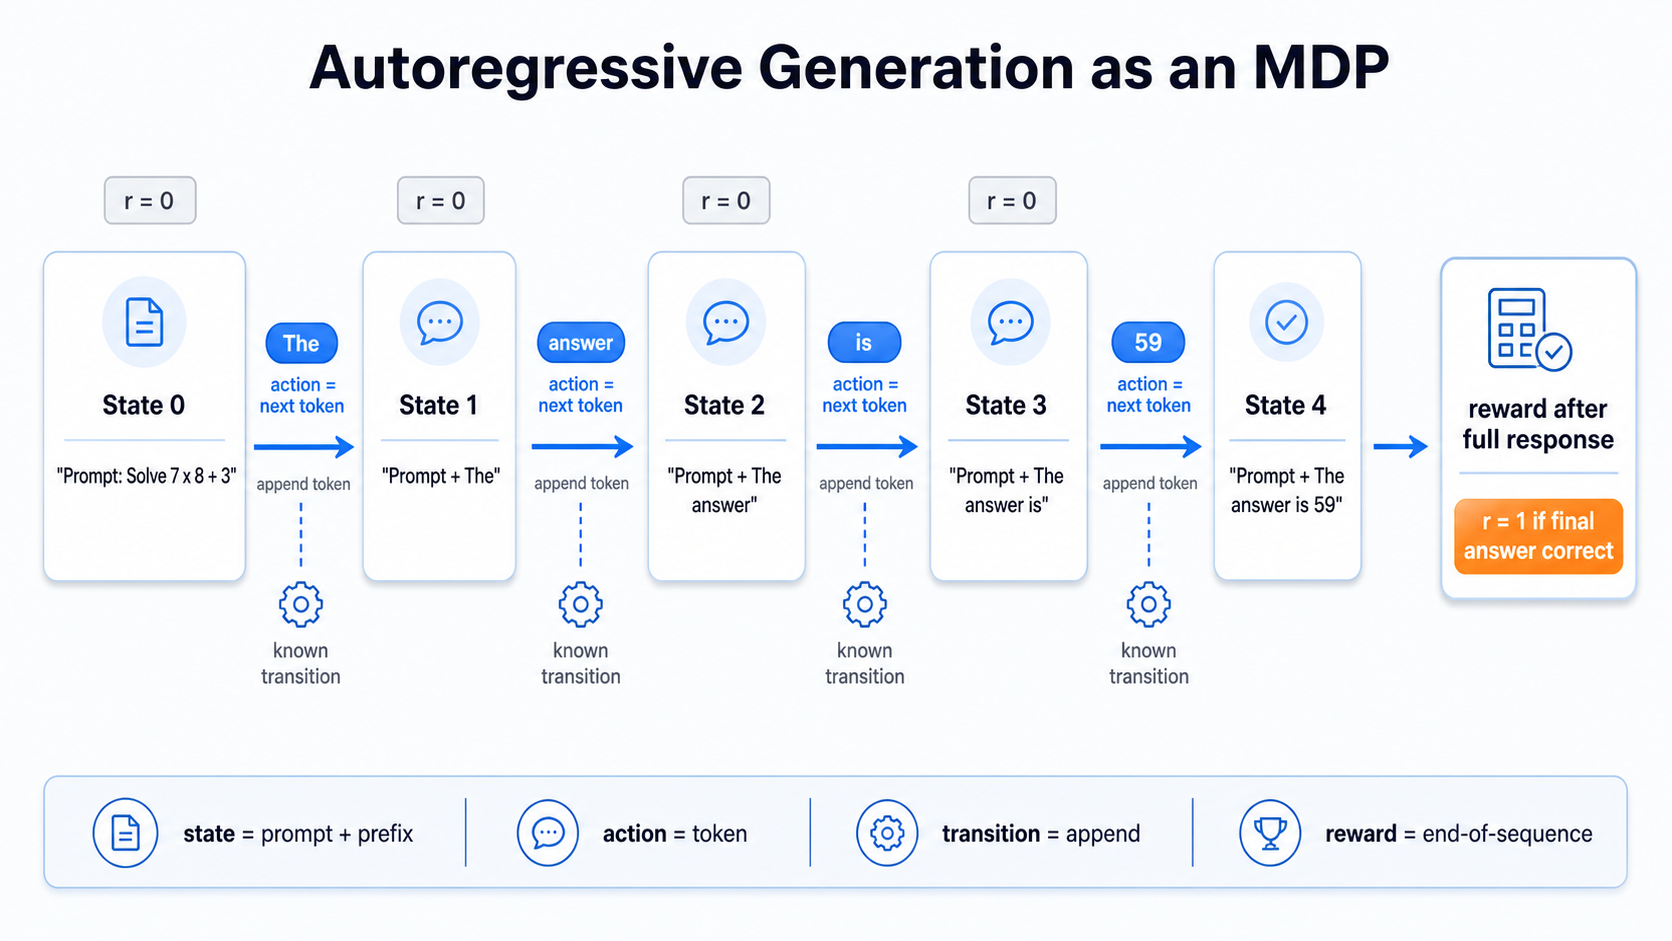
\includegraphics[width=0.95\textwidth]{figures/ch14/fig_llm_mdp.png}
\caption{\textbf{Language generation as a degenerate MDP.} Each state is the prompt plus tokens generated so far. Each action is the next token. Transitions are deterministic (appending the chosen token). Reward is sparse: zero at every intermediate step, assigned only after the complete response. The ``environment'' is trivial---all complexity lives in the policy (the language model itself).}
\label{fig:llm-mdp}
\end{figure}

\subsection{The Trajectory-Level Bandit Perspective}

These simplifications suggest an alternative framing. Instead of thinking of text generation as a 200-step sequential decision problem, think of it as a \textbf{single-step decision problem where the action is the entire response}:

\begin{itemize}[nosep]
  \item The ``state'' is the prompt $x$.
  \item The ``action'' is the complete response $y = (y_1, y_2, \ldots, y_T)$.
  \item The ``reward'' is $r(x, y)$---a scalar for the full response.
\end{itemize}

In this framing, LLM RL is a \textbf{contextual bandit}: the agent sees a context (prompt), takes a single action (generates a full response), and receives a reward. No sequential credit assignment needed. The complication, of course, is that the ``single action'' is exponentially large---the space of all possible responses. The policy factorizes this into per-token decisions via the chain rule:

\begin{equation}
\label{eq:trajectory-policy}
\pi_\theta(y \mid x) = \prod_{t=1}^{T} \pi_\theta(y_t \mid x, y_{<t})
\end{equation}

This factorization is what lets us use per-token policy gradients even though the reward is assigned at the trajectory level. It is also why the algorithms in this chapter work---they exploit the autoregressive structure to make gradient estimation tractable.

\begin{tcolorbox}[colback=blue!5, colframe=blue!40, title=\textbf{Is LLM RL ``Real'' RL?}]
Purists might object: if transitions are deterministic, reward is sparse, and the environment is trivial, is this really reinforcement learning? Technically, yes---it is a special case of the MDP framework, and the algorithms (REINFORCE, PPO) are standard RL algorithms. Practically, the simplifications are so extreme that LLM RL is closer to \emph{black-box optimization} than to the kind of RL that solves Atari or controls robots. The policy is the only interesting component; the ``environment'' is just string concatenation.

This is good news for you. It means that the RL machinery you need for Chapters~\ref{ch:rlhf} and~\ref{ch:reasoning-rl} is narrower than what a robotics RL course would teach. Model-based planning, multi-agent coordination, and sophisticated exploration theory are not the center of the story here. The load-bearing tools are policy gradients, variance reduction, clipped or regularized policy updates, and KL control. That is what the rest of this chapter provides.
\end{tcolorbox}

\begin{quickrecap}
\textbf{Quick Recap.}
\begin{itemize}[nosep,leftmargin=1.5em]
  \item LLM generation maps to an MDP with deterministic transitions, sparse end-of-sequence reward, and known dynamics.
  \item These simplifications make LLM RL narrower than general RL. The environment dynamics are known and deterministic; most uncertainty comes from the policy and the reward signal.
  \item Alternative framing: LLM RL is a contextual bandit where the action is the full response and the policy factorizes autoregressively.
\end{itemize}
\textit{Next: how to compute a gradient through a reward signal.}
\end{quickrecap}


%----------------------------------------------------------------------
\section{Policy Gradient}
\label{sec:policy-gradient}

You know how to compute gradients for supervised learning: define a loss, backpropagate. But in RL, there is no target output to compare against. The model generates a response, receives a scalar reward, and needs to adjust its parameters so that high-reward responses become more probable. The \textbf{policy gradient theorem} provides the mathematical tool for this.

\subsection{The Objective}

The RL objective is to maximize the expected reward under the policy:

\begin{equation}
\label{eq:rl-objective}
J(\theta) = \mathbb{E}_{y \sim \pi_\theta(\cdot \mid x)}\!\left[r(x, y)\right]
\end{equation}

We want $\nabla_\theta J(\theta)$---the direction in parameter space that increases expected reward. The challenge is that the expectation is over $\pi_\theta$ itself, which changes as we update $\theta$.

\subsection{The REINFORCE Estimator}

Williams (1992) showed that the policy gradient can be written as:

\begin{equation}
\label{eq:reinforce}
\nabla_\theta J(\theta) = \mathbb{E}_{y \sim \pi_\theta}\!\left[r(x, y) \; \nabla_\theta \log \pi_\theta(y \mid x)\right]
\end{equation}

\paragraph{Reading the equation.} The gradient has two factors:
\begin{itemize}[nosep]
  \item $\nabla_\theta \log \pi_\theta(y \mid x)$: the direction that makes response $y$ more likely.
  \item $r(x, y)$: how good that response was.
\end{itemize}

Multiply them together: the gradient pushes the policy toward high-reward responses (positive $r$) and away from low-reward responses (negative $r$). If all rewards are positive, the gradient pushes toward \emph{all} responses, but proportionally more toward the higher-reward ones.

\paragraph{Why this works.} The key insight is the \emph{log-derivative trick}: $\nabla_\theta \pi_\theta(y \mid x) = \pi_\theta(y \mid x) \, \nabla_\theta \log \pi_\theta(y \mid x)$. This allows us to move the gradient inside the expectation. We can estimate the gradient by sampling responses from the current policy, computing their rewards, and averaging. No backpropagation through the reward function is needed---the reward is a black box.

\paragraph{For autoregressive models.} Since $\pi_\theta(y \mid x) = \prod_t \pi_\theta(y_t \mid x, y_{<t})$, we have:

\begin{equation}
\label{eq:log-prob-decomp}
\log \pi_\theta(y \mid x) = \sum_{t=1}^{T} \log \pi_\theta(y_t \mid x, y_{<t})
\end{equation}

The log-probability is just the sum of per-token log-probabilities---the same quantity you already compute during SFT training. The REINFORCE gradient for your 3B model amounts to: sample a response, score it, then weight each token's log-probability gradient by the reward.

\subsection{The Variance Problem}

REINFORCE is unbiased but has catastrophically high variance. In practice, you might sample 8 responses to the same prompt: three get reward 1 (correct answer), five get reward 0. The gradient estimate from this batch is noisy because:

\begin{itemize}[nosep]
  \item A single high-reward response dominates the gradient. Its specific token choices---including irrelevant ones (``Let me think about this...'')---all get upweighted equally.
  \item The reward is trajectory-level, but the gradient is per-token. Credit assignment is implicit and noisy.
  \item If the reward variance is high, the gradient variance explodes.
\end{itemize}

Return to the cooking analogy: you make eight versions of a dish, and the critic gives scores. Three dishes score well. You try to learn from the winners, but you changed the spices, the temperature, \emph{and} the plating simultaneously. Which change mattered? Without a baseline (``how does an average dish score?''), every ingredient in the winning dishes gets equal credit---including the ones that were irrelevant. You need many trials to isolate what actually matters.

\subsection{Baselines and Advantage}

The standard fix is to subtract a \textbf{baseline} $b(x)$ from the reward:

\begin{equation}
\label{eq:reinforce-baseline}
\nabla_\theta J(\theta) = \mathbb{E}_{y \sim \pi_\theta}\!\left[(r(x, y) - b(x)) \; \nabla_\theta \log \pi_\theta(y \mid x)\right]
\end{equation}

The baseline does not change the expected gradient (it is unbiased for any $b$ that does not depend on $y$), but it dramatically reduces variance by centering the reward signal. The optimal baseline is the expected reward under the current policy---which is exactly the value function $V^\pi(x)$.

When we use $V^\pi$ as the baseline, the quantity $r(x, y) - V^\pi(x)$ is the \textbf{advantage}: how much better (or worse) this specific response was compared to the policy's average. Positive advantage: reinforce this response. Negative advantage: suppress it. Zero advantage: this response is exactly average, no gradient signal.

\begin{figure}[t]
\centering
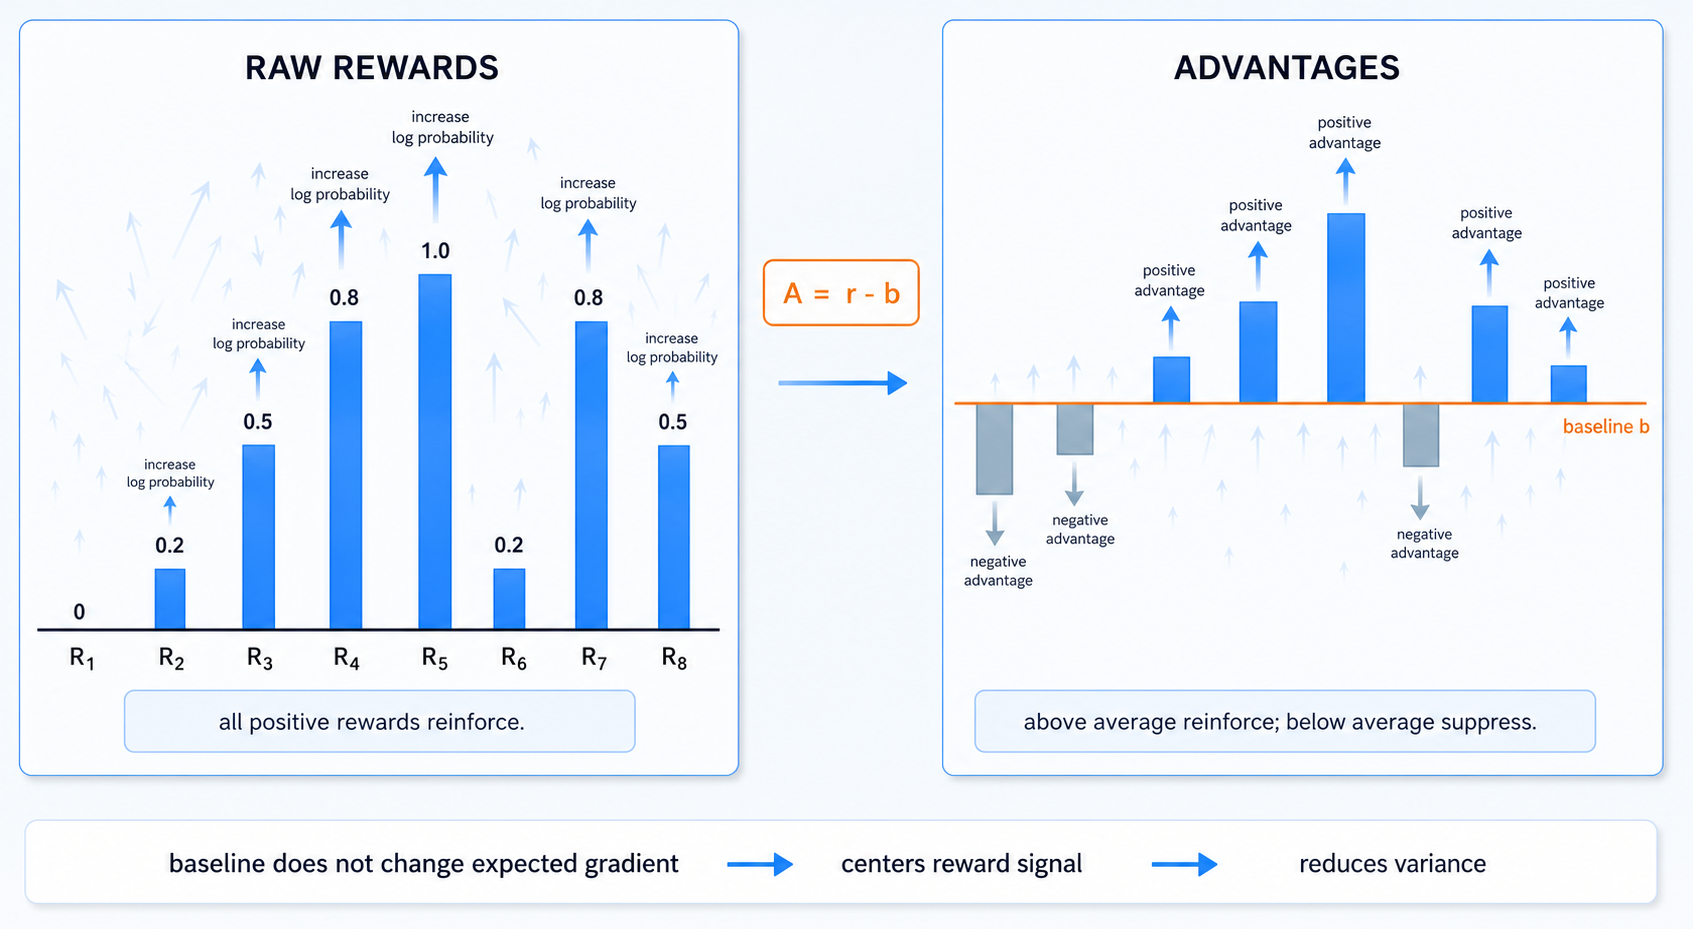
\includegraphics[width=0.95\textwidth]{figures/ch14/fig_reinforce_variance.png}
\caption{\textbf{Baselines reduce variance without changing the expected gradient.} Left: raw REINFORCE rewards for 8 sampled responses (all positive). All responses get upweighted, proportionally to reward. Right: after subtracting a baseline (the average reward), some responses have positive advantage (reinforce), others have negative advantage (suppress). The gradient signal is centered and more informative.}
\label{fig:reinforce-variance}
\end{figure}

\noindent\fbox{\parbox{\dimexpr\textwidth-2\fboxsep-2\fboxrule\relax}{%
\textbf{Pause and verify.} Your 3B model generates 4 responses to a math prompt. Rewards are $[1, 0, 1, 0]$ (correct/incorrect). The baseline is $b = 0.5$ (average reward). What are the advantages? Which responses get reinforced, which get suppressed? Now suppose all four rewards are $[1, 1, 1, 0]$ and $b = 0.75$. What changes? \emph{Notice that without the baseline, all three correct responses would be equally reinforced. With the baseline, the single incorrect response gets a strong negative signal ($-0.75$), while each correct response gets a mild positive signal ($+0.25$). The baseline makes failure informative.}
}}

\begin{quickrecap}
\textbf{Quick Recap.}
\begin{itemize}[nosep,leftmargin=1.5em]
  \item The REINFORCE estimator: weight each response's log-probability gradient by its reward.
  \item Raw REINFORCE has high variance because the reward is trajectory-level but the gradient is per-token.
  \item Subtracting a baseline (ideally the value function) reduces variance without introducing bias. The resulting signal is the advantage: how much better or worse than average.
\end{itemize}
\textit{Next: what happens when the policy that generated the data is not the policy you are updating.}
\end{quickrecap}


%----------------------------------------------------------------------
\section{Importance Sampling and Off-Policy Correction}
\label{sec:importance-sampling}

REINFORCE requires samples from the current policy $\pi_\theta$. But in practice, you generate a batch of responses, compute rewards (which may involve running a reward model or executing code), and \emph{then} update the policy. By the time you compute the gradient, $\pi_\theta$ has already moved---the samples were generated by a slightly older policy $\pi_{\theta_{\text{old}}}$.

\subsection{The Off-Policy Problem}

This is the \textbf{off-policy problem}: you are computing a gradient for $\pi_\theta$ using data generated by $\pi_{\theta_{\text{old}}}$. The standard correction is \textbf{importance sampling}:

\begin{equation}
\label{eq:importance-sampling}
\nabla_\theta J(\theta) = \mathbb{E}_{y \sim \pi_{\theta_{\text{old}}}}\!\left[\frac{\pi_\theta(y \mid x)}{\pi_{\theta_{\text{old}}}(y \mid x)} \; \hat{A}(x, y) \; \nabla_\theta \log \pi_\theta(y \mid x)\right]
\end{equation}

The ratio $\rho = \pi_\theta(y \mid x) / \pi_{\theta_{\text{old}}}(y \mid x)$ corrects for the distributional mismatch. If $\pi_\theta$ and $\pi_{\theta_{\text{old}}}$ are identical, $\rho = 1$ and we recover standard REINFORCE. If they diverge, $\rho$ reweights each sample: a response that the new policy finds more likely than the old one gets amplified ($\rho > 1$); a response the new policy finds less likely gets downweighted ($\rho < 1$).

\paragraph{Concretely.} Suppose your 3B model generates the response ``The answer is 56'' to a math prompt. Under the old policy, this response had probability $0.03$. After one gradient step, the new policy assigns probability $0.06$. The importance ratio is $\rho = 0.06 / 0.03 = 2.0$---this sample counts twice as much in the gradient, because the new policy ``likes'' it more than the old one did.

\subsection{Why Importance Ratios Explode for LLMs}

Large importance ratios amplify gradient noise. If a response was unlikely under $\pi_{\theta_{\text{old}}}$ but likely under $\pi_\theta$, the ratio $\rho$ can be $10\times$ or $100\times$, making that single sample dominate the entire gradient. In the worst case, a single outlier ratio destabilizes training.

The problem is especially severe for language models. Recall that $\pi_\theta(y \mid x) = \prod_t \pi_\theta(y_t \mid x, y_{<t})$ (Equation~\ref{eq:log-prob-decomp}). The sequence-level ratio is therefore a \emph{product} of per-token ratios:

\[
\rho = \prod_{t=1}^{T} \frac{\pi_\theta(y_t \mid x, y_{<t})}{\pi_{\theta_{\text{old}}}(y_t \mid x, y_{<t})}
\]

Even small per-token changes compound. A per-token ratio of 1.05 means the new policy assigns 5\% more probability to that token---barely noticeable for any single token. But for a 200-token response: $1.05^{200} \approx 17{,}000$. This one sample would dominate a batch of thousands. This is why naively applying importance sampling to LLMs fails catastrophically, and why PPO's clipping mechanism (\S\ref{sec:ppo}) is essential.

\begin{quickrecap}
\textbf{Quick Recap.}
\begin{itemize}[nosep,leftmargin=1.5em]
  \item Off-policy problem: data generated by an old policy, gradient computed for the current policy.
  \item Importance sampling corrects the distributional mismatch via the probability ratio $\rho$.
  \item For long sequences, $\rho$ can explode due to compounding per-token ratios. Unconstrained importance sampling is impractical for LLMs.
\end{itemize}
\textit{Next: the algorithm that tames this instability.}
\end{quickrecap}


%----------------------------------------------------------------------
\section{PPO}
\label{sec:ppo}

Proximal Policy Optimization (Schulman et al., 2017)~\cite{schulman2017ppo} is the workhorse algorithm behind classical RLHF (Chapter~\ref{ch:rlhf}) and the reference point for many later reasoning-RL variants (Chapter~\ref{ch:reasoning-rl}). It addresses the importance-sampling variance problem from \S\ref{sec:importance-sampling} with a simple mechanism: clip the probability ratio so it cannot deviate too far from 1.

\subsection{TRPO Intuition: The Trust Region}

Before PPO, there was TRPO (Trust Region Policy Optimization)~\cite{schulman2015trpo}. TRPO's insight: if you constrain each policy update so that $\pi_\theta$ stays close to $\pi_{\theta_{\text{old}}}$ (measured by KL divergence), you can guarantee monotonic improvement. The problem is that TRPO enforces this constraint via a second-order optimization step---computing the Fisher information matrix and solving a constrained optimization problem. This is expensive and complicated to implement.

PPO replaces TRPO's hard KL constraint with a soft clipping mechanism that achieves a similar effect with standard first-order optimization. In the cooking analogy: TRPO says ``you may only change your recipe by this much per iteration''; PPO says ``change whatever you want, but once you have changed any ingredient by more than 20\%, stop getting credit for further changes to that ingredient.''

\subsection{The Clipped Surrogate Objective}

The PPO objective is:

\begin{equation}
\label{eq:ppo-clip}
\mathcal{L}^{\text{PPO}}(\theta) = \mathbb{E}\!\left[\min\!\left(\rho_t \, \hat{A}_t, \;\; \text{clip}(\rho_t, 1-\epsilon, 1+\epsilon) \, \hat{A}_t\right)\right]
\end{equation}

where $\rho_t = \pi_\theta(a_t \mid s_t) / \pi_{\theta_{\text{old}}}(a_t \mid s_t)$ and $\epsilon$ is a small constant (typically 0.1--0.2).

\paragraph{How clipping works.} Two cases:

\begin{itemize}[nosep]
  \item \textbf{Positive advantage ($\hat{A}_t > 0$)}: the action was better than average. The objective encourages increasing $\rho_t$ (making this action more likely). But the clip caps $\rho_t$ at $1 + \epsilon$. Once the policy has increased the probability by factor $1 + \epsilon$ relative to the old policy, there is no further gradient. The policy cannot ``overshoot.''
  \item \textbf{Negative advantage ($\hat{A}_t < 0$)}: the action was worse than average. The objective encourages decreasing $\rho_t$. The clip caps $\rho_t$ at $1 - \epsilon$. Once the probability has decreased by factor $1 - \epsilon$, there is no further gradient. The policy cannot suppress this action too aggressively.
\end{itemize}

The $\min$ operator selects the more conservative estimate. This creates a ``trust region'' without second-order optimization: the policy can change, but not too much per update.

\begin{figure}[t]
\centering
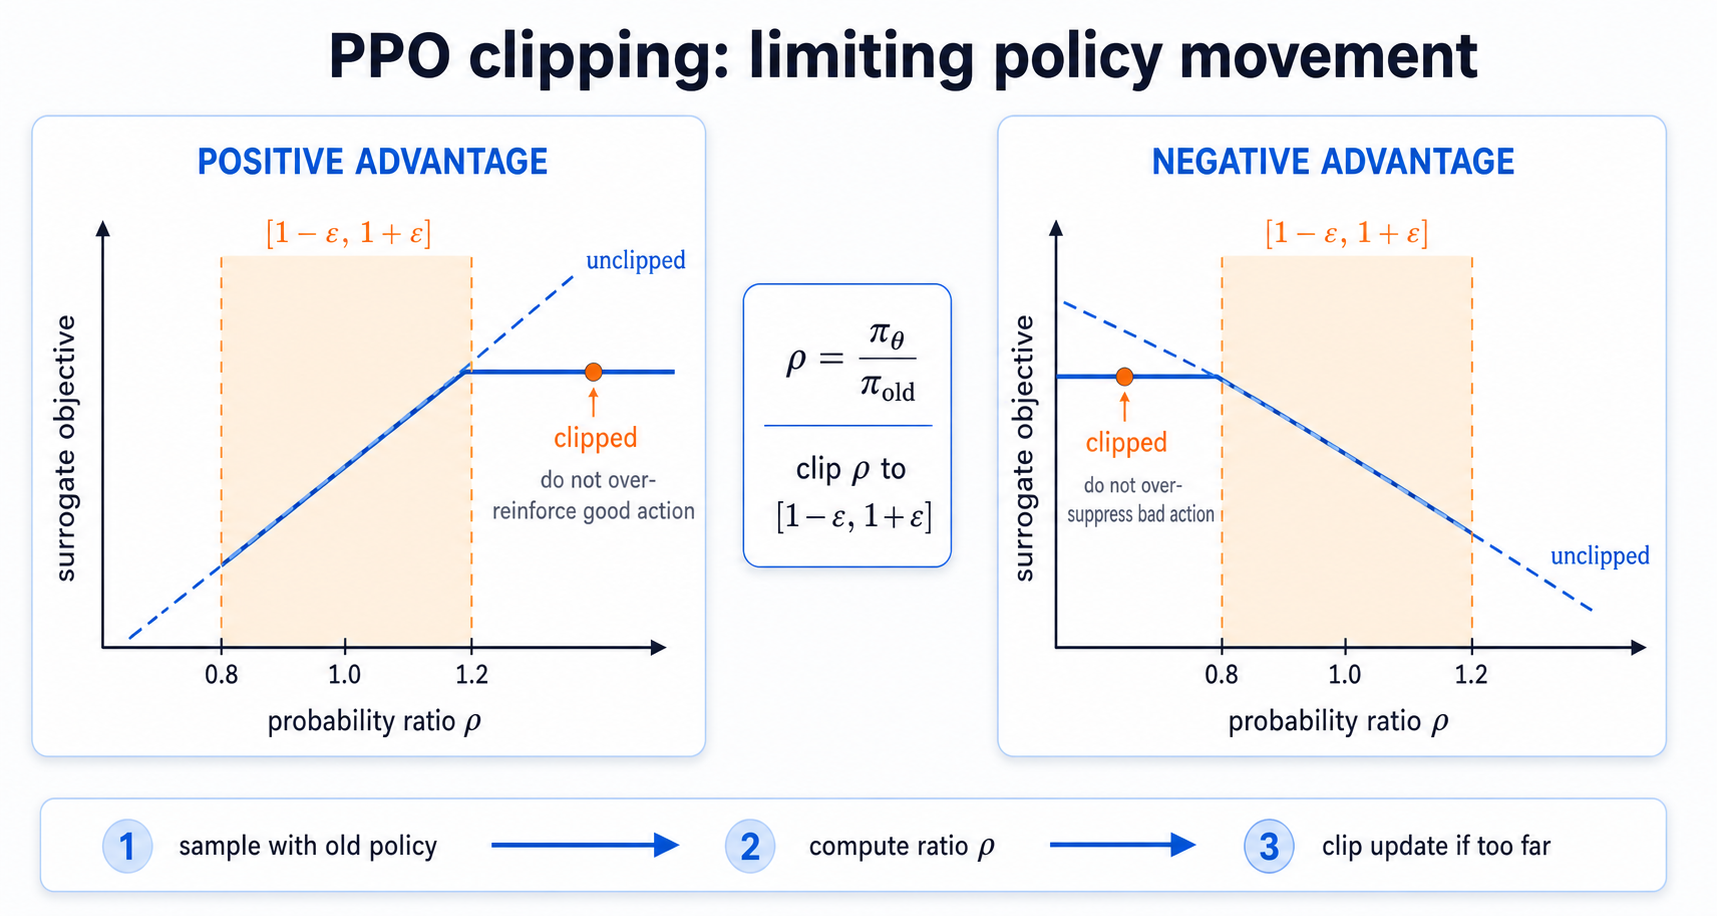
\includegraphics[width=0.95\textwidth]{figures/ch14/fig_ppo_clipping.png}
\caption{\textbf{PPO's clipping mechanism.} The objective as a function of the probability ratio $\rho$ for positive advantage (left) and negative advantage (right). The unclipped objective (dashed line) grows without bound as $\rho$ increases or decreases. The clipped objective (solid line) becomes flat outside the interval $[1-\epsilon, 1+\epsilon]$, creating a ``trust region'' where the sample stops receiving extra credit for further policy movement.}
\label{fig:ppo-clipping}
\end{figure}

\subsection{Generalized Advantage Estimation (GAE)}

The advantage $\hat{A}_t$ in Equation~\ref{eq:ppo-clip} needs to be estimated. In standard RL with per-step rewards, \textbf{Generalized Advantage Estimation} (GAE)~\cite{schulman2016gae} computes the advantage as an exponentially weighted average of $n$-step returns:

\begin{equation}
\label{eq:gae}
\hat{A}_t^{\text{GAE}} = \sum_{l=0}^{T-t} (\gamma \lambda)^l \, \delta_{t+l}, \quad \text{where} \quad \delta_t = r_t + \gamma V(s_{t+1}) - V(s_t)
\end{equation}

The parameter $\lambda \in [0, 1]$ trades off bias and variance: $\lambda = 0$ gives the one-step TD residual (low variance, high bias), $\lambda = 1$ gives the full Monte Carlo return (high variance, low bias).

\paragraph{GAE for LLMs.} In the standard LLM-RL setup with end-of-sequence reward only, intermediate rewards $r_t$ are zero for all $t < T$. GAE simplifies: the advantage at each token is determined by the difference between the eventual reward and the value function's prediction. In practice, the value model (a separate network or a head on the policy) learns to predict the expected reward from any partial sequence. GRPO (Chapter~\ref{ch:reasoning-rl}) avoids the value model entirely by using a simpler group-level baseline, but the PPO-based RLHF systems in Chapter~\ref{ch:rlhf} use GAE with a learned value function.

\subsection{PPO in Practice}

A typical PPO training step for LLMs:

\begin{enumerate}[nosep]
  \item \textbf{Rollout}: sample a batch of prompts, generate responses with $\pi_{\theta_{\text{old}}}$.
  \item \textbf{Score}: compute reward for each response (reward model, verifier, or unit tests).
  \item \textbf{Advantage}: estimate $\hat{A}_t$ using GAE (or a simpler baseline).
  \item \textbf{Update}: take $K$ gradient steps on the PPO-clip objective (Equation~\ref{eq:ppo-clip}), typically $K = 4$.
  \item \textbf{Replace}: set $\pi_{\theta_{\text{old}}} \leftarrow \pi_\theta$ and repeat.
\end{enumerate}

\paragraph{For Project~3.} If you were to use PPO on your 3B model with a math verifier: generate 8 responses per prompt, score each with the verifier (1 = correct, 0 = incorrect), compute advantages (correct responses get positive advantage, incorrect get negative), and update the policy for 4 mini-batch epochs with clip $\epsilon = 0.2$. The clipping ensures that even if one correct response has an unusually high log-probability ratio, it does not keep receiving extra credit once the policy has moved beyond the trust region.

\noindent\fbox{\parbox{\dimexpr\textwidth-2\fboxsep-2\fboxrule\relax}{%
\textbf{Pause and verify.} In the PPO objective (Equation~\ref{eq:ppo-clip}), suppose $\hat{A}_t > 0$ and $\rho_t = 1.3$ with $\epsilon = 0.2$. The unclipped term is $1.3 \times \hat{A}_t$. The clipped term is $\text{clip}(1.3, 0.8, 1.2) \times \hat{A}_t = 1.2 \times \hat{A}_t$. The $\min$ selects $1.2 \times \hat{A}_t$. \emph{This sample no longer receives additional objective value from increasing $\rho_t$ further}---the policy has already moved past the trust region for this action. This is PPO's stabilizing effect: extreme probability-ratio changes stop dominating the update.
}}

\begin{quickrecap}
\textbf{Quick Recap.}
\begin{itemize}[nosep,leftmargin=1.5em]
  \item PPO clips the importance sampling ratio to $[1-\epsilon, 1+\epsilon]$, preventing large policy updates.
  \item The $\min$ operator selects the more conservative estimate: the clipped or unclipped surrogate, whichever gives less credit.
  \item GAE estimates advantages by blending TD residuals across time steps. For LLMs with end-of-sequence reward, it simplifies via the value model.
  \item PPO is the standard algorithm behind classical RLHF and the reference point for later critic-free variants such as GRPO.
\end{itemize}
\textit{Next: the additional constraint that LLM RL specifically requires.}
\end{quickrecap}


%----------------------------------------------------------------------
\section{KL Constraint to Reference Policy}
\label{sec:kl-rl}

Standard RL aims to maximize reward without limit. If the reward model gives high scores to verbose, repetitive responses (because verbose answers superficially look more thorough), an unconstrained policy will exploit this: responses grow to maximum length, filled with hedging phrases and restatements. The model has found a ``reward hack''---a strategy that scores well on the proxy (reward model) while being useless to humans.

In the cooking analogy, the food critic is a proxy for actual diners. Near your current style of cooking, the critic's scores correlate well with diner satisfaction. But if you optimize the critic's scoring rubric aggressively---say, discovering that the critic always gives bonus points for truffle oil---you end up with dishes that score 10/10 on the rubric but that no real diner would enjoy. The KL constraint says: keep cooking roughly the way you already know how, and improve from there.

More generally, when you optimize a proxy for a true objective, the proxy breaks down at the extremes (Goodhart's law, which Chapter~\ref{ch:evaluation} discussed in the context of benchmarks). In LLM RL, the fix is a \textbf{KL penalty} to a frozen reference policy $\pi_{\text{ref}}$ (typically the SFT checkpoint):

\begin{equation}
\label{eq:kl-rl-objective}
J_{\text{KL}}(\theta) = \mathbb{E}_{y \sim \pi_\theta}\!\left[r(x, y)\right] - \beta \, D_{\text{KL}}\!\left[\pi_\theta(\cdot \mid x) \;\|\; \pi_{\text{ref}}(\cdot \mid x)\right]
\end{equation}

\begin{tcolorbox}[colback=gray!8, colframe=gray!40]
\textbf{Echo: the KL-constrained objective.} You have seen this equation before. In Chapter~\ref{ch:preference-learning} \S\ref{sec:kl-objective}, we introduced the same objective as ``an optimization problem, not an RL problem'' and derived its closed-form solution---which led to DPO. Now you see where the objective comes from: it is the natural RL objective with a regularization term that prevents the policy from drifting too far from the reference. In DPO, you solve it in closed form and avoid RL entirely. In RLHF (Chapter~\ref{ch:rlhf}), you optimize it directly with PPO. Same objective, two different optimization strategies.
\end{tcolorbox}

\subsection{Why the KL Penalty Is Essential}

The KL penalty serves three purposes:

\begin{enumerate}[nosep]
  \item \textbf{Reward hacking prevention.} The reward model is an imperfect proxy for human preferences. Near the SFT policy, the proxy is well-calibrated (the RM was trained on data from policies close to SFT). Far from SFT, the proxy becomes unreliable---it assigns high reward to responses it has never seen during training. The KL constraint keeps the policy in the region where the reward model is trustworthy.
  \item \textbf{Capability preservation.} The pretrained model has broad language competence. Without KL, the policy can ``forget'' how to do basic generation in pursuit of reward. The reference anchor preserves the base capabilities while allowing targeted improvement.
  \item \textbf{Diversity maintenance.} Without KL, the policy tends to collapse to a single high-reward response template (mode collapse). The KL penalty maintains distributional diversity by penalizing deviations from the reference's spread.
\end{enumerate}

\paragraph{What happens without KL.} Suppose you train your 3B model with a learned reward model and set $\beta = 0$ (no KL penalty). Within a few hundred steps, you observe predictable pathologies:

\begin{itemize}[nosep]
  \item Response length grows monotonically if the reward model slightly favors longer-looking responses.
  \item Entropy drops (the policy converges to a small set of high-reward templates).
  \item Reward increases but human preference decreases---the classic over-optimization signature from Gao et al.~\cite{gao2023scaling}.
  \item After enough training, the model can produce fluent-sounding gibberish that scores well on the reward model but is unhelpful or nonsensical to humans.
\end{itemize}

With a hard verifier, such as exact-answer math checking, the failure mode is different but the lesson is the same: if the verifier or answer extractor has loopholes, an unconstrained policy will search for them. If the verifier is genuinely exact, KL still helps preserve the model's language quality, format discipline, and diversity while the policy learns to exploit the outcome signal.

\begin{figure}[t]
\centering
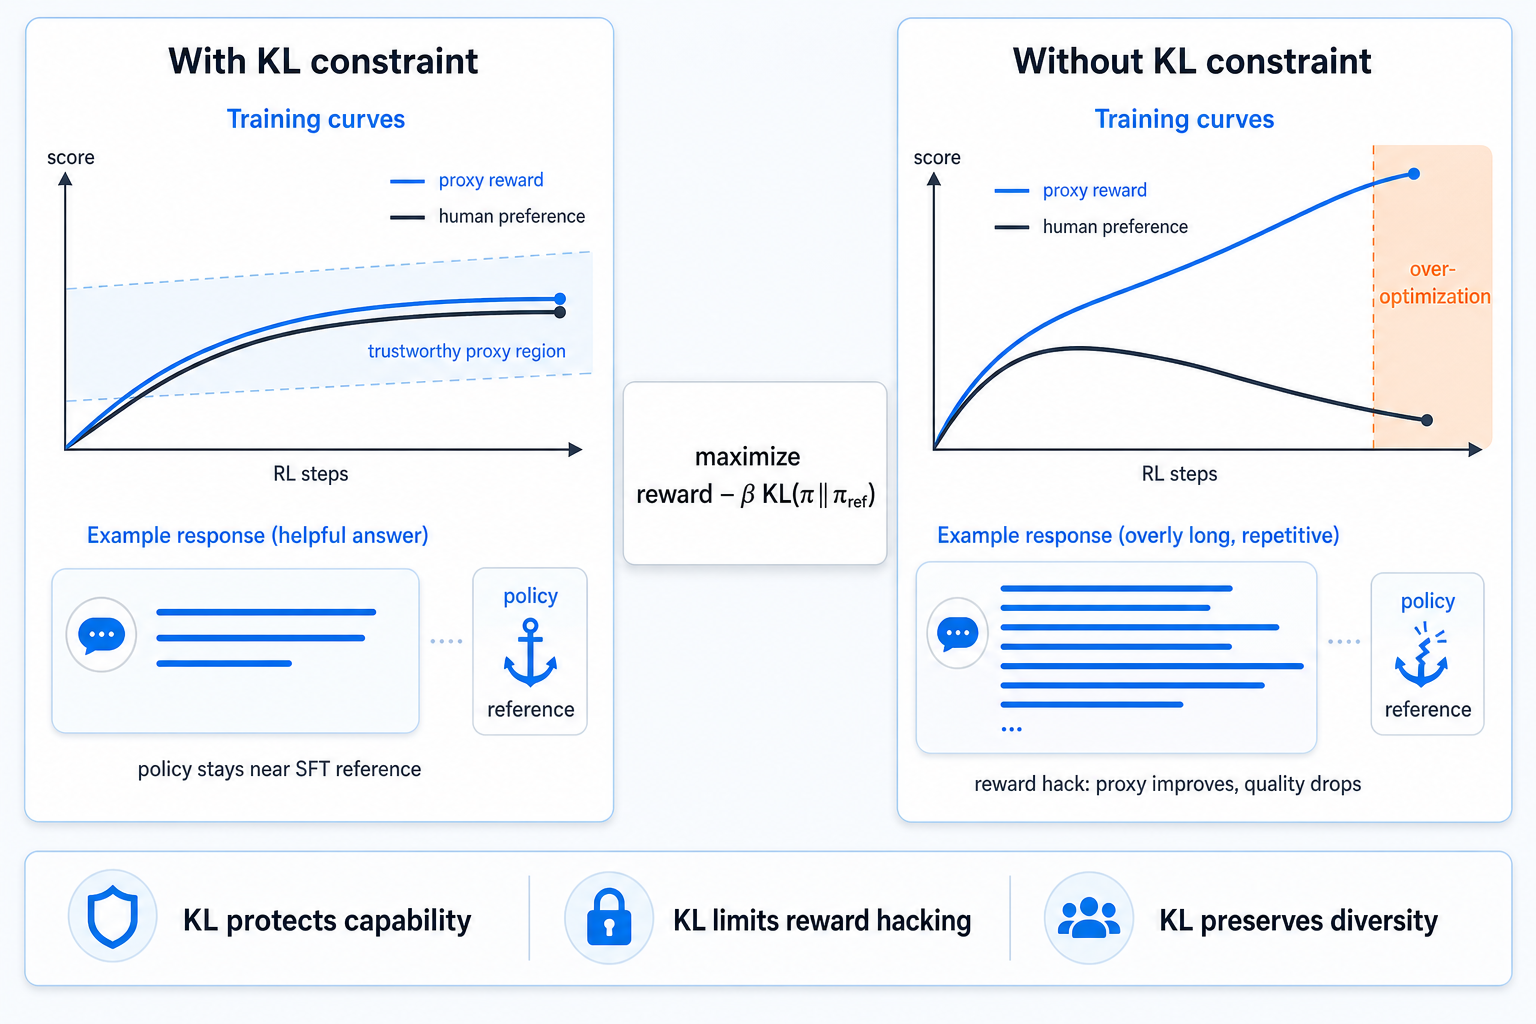
\includegraphics[width=0.95\textwidth]{figures/ch14/fig_kl_constraint.png}
\caption{\textbf{The effect of KL constraint on RLHF training.} Left: with KL constraint ($\beta > 0$), the policy improves reward while staying close to the reference. Reward increases moderately and then plateaus; human preference also improves. Right: without KL constraint ($\beta = 0$), reward increases rapidly (the policy exploits the reward model), but human preference peaks early and then degrades as the policy enters the over-optimization regime. The KL penalty keeps the policy in the ``trustworthy proxy'' region.}
\label{fig:kl-constraint}
\end{figure}

\subsection{In Practice: KL Coefficient Scheduling}

The coefficient $\beta$ in Equation~\ref{eq:kl-rl-objective} is a critical hyperparameter:

\begin{itemize}[nosep]
  \item \textbf{Too large}: the policy barely moves from the reference. You are paying the cost of RL (rollouts, scoring, PPO updates) for negligible improvement.
  \item \textbf{Too small}: the policy over-optimizes the reward model. You get high proxy reward but low actual quality.
\end{itemize}

Some implementations use \textbf{adaptive KL}: set a target KL divergence (e.g., 6 nats), and adjust $\beta$ dynamically to keep $D_{\text{KL}}[\pi_\theta \| \pi_{\text{ref}}]$ near this target. When the KL is too high, increase $\beta$ (slow down). When it is too low, decrease $\beta$ (allow more exploration). InstructGPT used this adaptive scheme~\cite{ouyang2022instructgpt}.

\begin{tcolorbox}[colback=orange!5, colframe=orange!60, title=\textbf{For Project~3: KL in Practice}]
If you use PPO to train your 3B model on math verification rewards:
\begin{itemize}[nosep]
  \item Start with $\beta = 0.05$ and target KL $\approx 5$--$10$.
  \item Monitor KL divergence per batch. If it exceeds 15, the policy is drifting too fast---increase $\beta$ or reduce the learning rate.
  \item A simple sanity check: generate from both $\pi_\theta$ and $\pi_{\text{ref}}$ on the same prompts. If $\pi_\theta$'s outputs look qualitatively different (different style, much longer, repetitive), the KL is too high.
\end{itemize}
\end{tcolorbox}

\begin{quickrecap}
\textbf{Quick Recap.}
\begin{itemize}[nosep,leftmargin=1.5em]
  \item The KL penalty to the reference policy prevents reward hacking, preserves capability, and maintains diversity.
  \item Without KL, RL training over-optimizes the reward model proxy: high reward but low human preference.
  \item The same KL-constrained objective appeared in Chapter~\ref{ch:preference-learning}'s DPO derivation. DPO solves it in closed form; RLHF optimizes it with PPO.
  \item $\beta$ can be fixed or adaptive (target a KL budget per batch).
\end{itemize}
\textit{Next: what this chapter deliberately did not cover.}
\end{quickrecap}


%----------------------------------------------------------------------
\section{The Broader RL Landscape}
\label{sec:rl-not-covered}

This chapter developed the minimum RL vocabulary for Chapters~\ref{ch:rlhf} and~\ref{ch:reasoning-rl}: MDP formalism, the LLM-as-degenerate-MDP insight, REINFORCE, importance sampling, PPO, and KL-constrained optimization. That is the complete toolkit for understanding RLHF and reasoning RL as practiced in 2022--2026.

But RL as a field is far broader. Understanding what we \emph{did} cover is easier when you see what we did not---and why those pieces are less central to the LLM post-training story:

\begin{figure}[t]
\centering
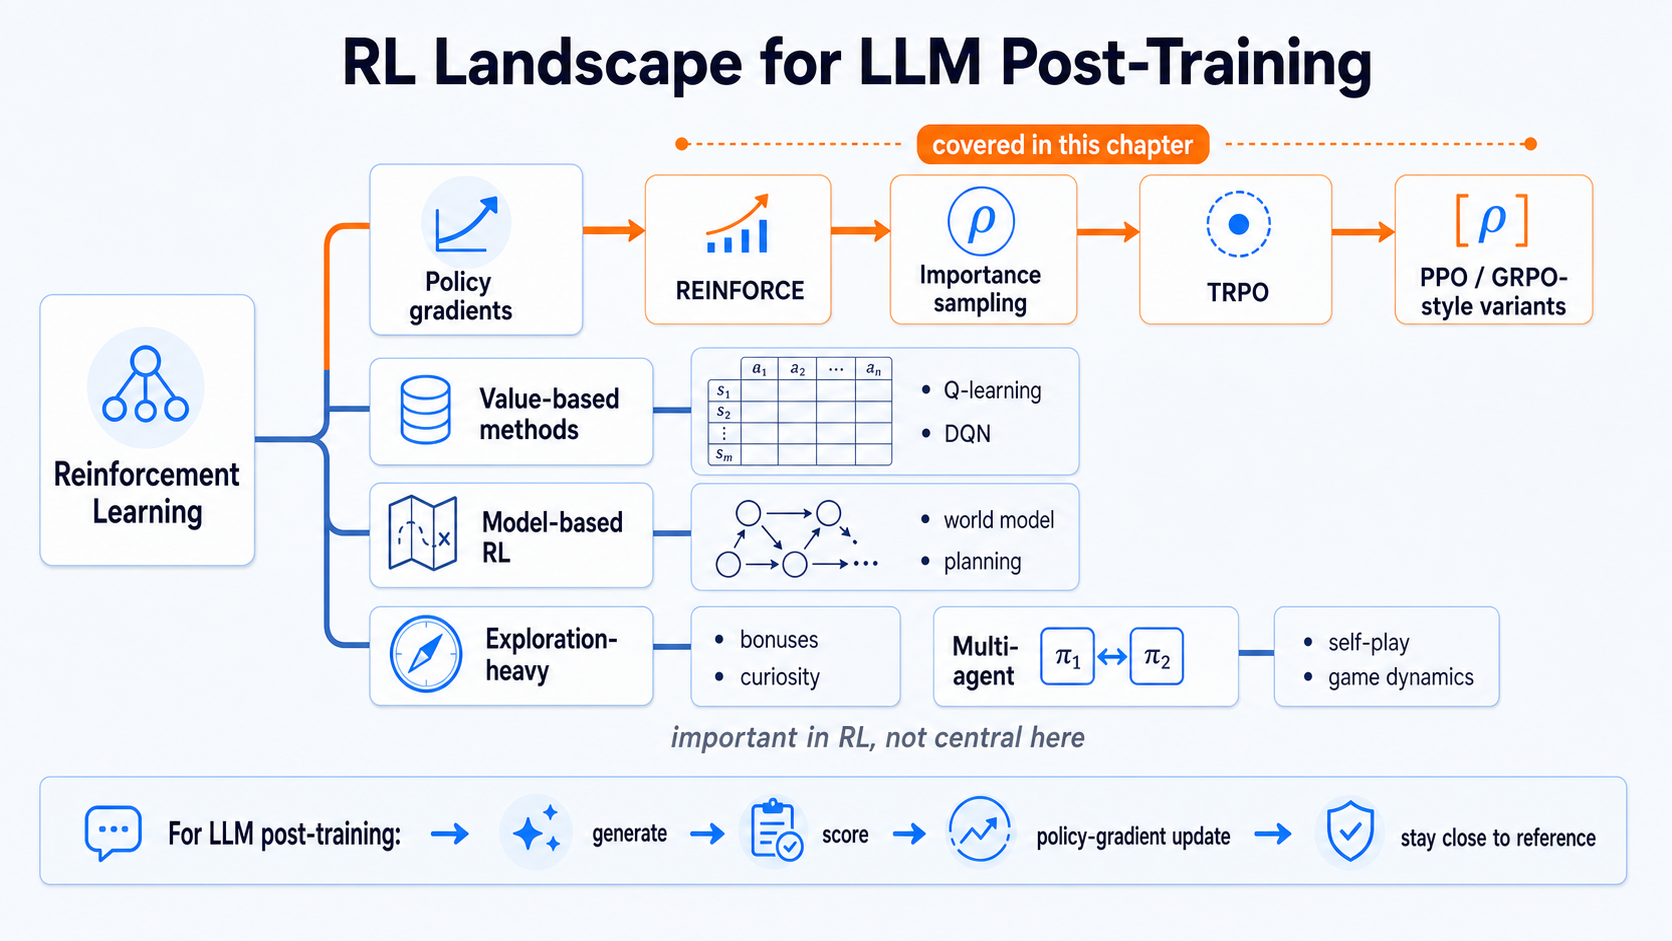
\includegraphics[width=0.95\textwidth]{figures/ch14/fig_rl_landscape.png}
\caption{\textbf{The RL landscape: what we covered vs.\ what exists.} This chapter covered the policy-gradient family (REINFORCE $\to$ TRPO $\to$ PPO), which is the branch most directly used in LLM RLHF and reasoning-RL systems. Value-based methods (Q-learning, DQN), model-based methods (world models, planning), and multi-agent RL are important elsewhere in RL, but they are not central to the post-training pipeline this part of the book studies.}
\label{fig:rl-landscape}
\end{figure}

\begin{itemize}[nosep]
  \item \textbf{Value-based methods (Q-learning, DQN).} These learn a value function and derive a policy from it. They work well for discrete, low-dimensional action spaces (Atari) but are impractical for vocabulary-sized action spaces (50{,}000+ tokens).
  \item \textbf{Model-based RL.} Learns a model of the environment and uses it for planning. Unnecessary for LLM RL because the environment (token concatenation) is already known.
  \item \textbf{Exploration theory.} Classical RL struggles with exploration---how to visit new states when the agent does not know what is rewarding. LLM RL has a natural first mechanism: sampling from the policy. Temperature, top-$p$, and generating multiple responses per prompt provide diversity. This does not make exploration solved, especially for hard reasoning tasks; it only means that exploration is not the organizing problem for this chapter's core algorithms.
  \item \textbf{Multi-agent RL.} Not currently used in post-training, though self-play (Chapter~\ref{ch:frontiers}) involves related ideas.
  \item \textbf{Offline RL.} Learning from a fixed dataset without further environment interaction. DPO (Chapter~\ref{ch:preference-learning}) can be viewed as a form of offline RL, but the connection is not central to this course.
  \item \textbf{Temporal credit assignment in detail.} With sparse end-of-sequence reward, credit assignment is a real challenge. Process reward models (Chapter~\ref{ch:reasoning-rl}) are one approach, but a full treatment of credit assignment is beyond our scope.
\end{itemize}

\paragraph{Where to go deeper.} Three resources:

\begin{enumerate}[nosep]
  \item Sutton \& Barto, \emph{Reinforcement Learning: An Introduction} (2nd edition). The canonical RL textbook. Chapters 2--5 (bandits, MDPs, dynamic programming) and 13 (policy gradient) are most relevant.
  \item Levine, UC Berkeley CS 285 (Deep RL). Lecture notes and videos available online. Comprehensive coverage of policy gradients, actor-critic methods, and model-based RL.
  \item Achiam, \emph{Spinning Up in Deep RL} (OpenAI). A practical introduction with clean implementations. Good for building intuition before diving into theory.
\end{enumerate}

This chapter gave you the vocabulary for Chapters~\ref{ch:rlhf} and~\ref{ch:reasoning-rl}. A full RL course would give you much more---but what you have now is enough to read any RLHF or reasoning-RL paper published between 2022 and 2026.

\begin{quickrecap}
\textbf{Quick Recap.}
\begin{itemize}[nosep,leftmargin=1.5em]
  \item This chapter covered the policy-gradient family: REINFORCE $\to$ importance sampling $\to$ PPO-style clipped updates.
  \item We omitted value-based methods, model-based RL, exploration theory, and multi-agent RL because they are not central to the post-training methods in Chapters~\ref{ch:rlhf} and~\ref{ch:reasoning-rl}.
  \item Sutton \& Barto, CS 285, and Spinning Up are the recommended next steps for readers who want deeper RL knowledge.
\end{itemize}
\end{quickrecap}


%----------------------------------------------------------------------
% End matter
%----------------------------------------------------------------------

\begin{takeaways}
\begin{enumerate}
  \item RL learns from reward signals, not demonstrations or preferences. It is needed when the desired behavior cannot be demonstrated or when evaluation is objective but solutions are creative.
  \item An MDP formalizes sequential decision-making with states, actions, transitions, rewards, and a discount factor. The goal is to maximize expected return.
  \item Autoregressive text generation is a degenerate MDP: deterministic transitions, sparse end-of-sequence reward, known dynamics. Most of classical RL's complexity disappears.
  \item The REINFORCE estimator converts a reward signal into a policy gradient. It is unbiased but high-variance. Baselines (especially the value function) reduce variance by centering the reward signal.
  \item PPO clips the importance sampling ratio to prevent large policy updates, achieving trust-region-like stability with simple first-order optimization.
  \item The KL penalty to a reference policy prevents reward hacking, preserves capability, and maintains output diversity. It is the same objective that underlies DPO (Chapter~\ref{ch:preference-learning}).
\end{enumerate}
\end{takeaways}


\section*{Summary}

\paragraph{What this chapter established.} Starting from the general MDP framework, we showed that autoregressive text generation is a degenerate special case---deterministic transitions, sparse reward, known dynamics---where the relevant RL toolkit is much narrower than in robotics or games. We developed the minimum viable toolkit: the REINFORCE gradient estimator for converting reward to parameter updates, importance sampling for off-policy correction, and PPO's clipping mechanism for stable training. We then introduced the KL constraint to a reference policy---the same constraint that appeared in Chapter~\ref{ch:preference-learning}'s DPO derivation---and explained why it is essential for preventing reward hacking.

\paragraph{The degenerate-MDP insight.} The central lesson of this chapter is that LLM RL is narrower than general RL. The formalism is inherited from a field that solves robotic control and game playing, but the application removes several sources of difficulty. Transitions are deterministic, so you do not need to learn a dynamics model. The environment is known, and sampling from the policy gives a direct way to explore candidate responses. The action space is large but discrete, so policy gradients apply directly to token probabilities. What remains is the core loop from the opening analogy: cook a dish (generate a response), get a score (reward), adjust your technique (policy gradient), and stay close to what you already know works (KL constraint). This is why PPO-style policy optimization has been the stable center of LLM RL since 2022, even as newer variants simplify or replace pieces of the PPO stack.

\paragraph{One sentence.} \emph{RL for language models is policy-gradient optimization over a deterministic token-generation process, regularized by a KL constraint that keeps the model cooking roughly the way it already knows---improving from there, not reinventing from scratch.}

\paragraph{What comes next.} Chapter~\ref{ch:rlhf} instantiates this machinery on the RLHF pipeline: a learned reward model scores responses, PPO updates the policy, and the KL constraint prevents over-optimization. You will see the InstructGPT three-stage pipeline in full technical detail. Chapter~\ref{ch:reasoning-rl} then replaces the learned reward model with verifiable rewards (math correctness, code tests) and replaces PPO's value model with a simpler group-level baseline (GRPO). Different reward sources, same policy-gradient spine.


\section*{Key Equations at a Glance}

\begin{center}
\begin{tabularx}{\textwidth}{@{}lX@{}}
\toprule
\textbf{Name} & \textbf{Equation} \\
\midrule
REINFORCE gradient & $\nabla_\theta J = \mathbb{E}_{y \sim \pi_\theta}\!\left[(r(x,y) - b) \, \nabla_\theta \log \pi_\theta(y \mid x)\right]$ \\[6pt]
PPO-clip objective & $\mathcal{L}^{\text{PPO}} = \mathbb{E}\!\left[\min\!\left(\rho_t \hat{A}_t, \; \text{clip}(\rho_t, 1{-}\epsilon, 1{+}\epsilon) \hat{A}_t\right)\right]$ \\[6pt]
KL-constrained objective & $J_{\text{KL}} = \mathbb{E}_{y \sim \pi_\theta}\!\left[r(x,y)\right] - \beta \, D_{\text{KL}}\!\left[\pi_\theta \| \pi_{\text{ref}}\right]$ \\[6pt]
GAE advantage & $\hat{A}_t^{\text{GAE}} = \sum_{l=0}^{T-t}(\gamma\lambda)^l \delta_{t+l}$, \quad $\delta_t = r_t + \gamma V(s_{t+1}) - V(s_t)$ \\
\bottomrule
\end{tabularx}
\end{center}


\section*{Key Readings}

\begin{enumerate}[nosep]
  \item \textbf{Schulman et al., 2017.} ``Proximal Policy Optimization Algorithms'' (PPO). The algorithm behind classical RLHF and the reference point for later LLM RL variants. Short paper, clearly written. Read for the clipping mechanism and the practical design choices.
  \item \textbf{Williams, 1992.} ``Simple Statistical Gradient-Following Algorithms for Connectionist Reinforcement Learning'' (REINFORCE). The foundational policy gradient algorithm. Read for the derivation of the log-derivative trick.
  \item \textbf{Schulman et al., 2016.} ``High-Dimensional Continuous Control Using Generalized Advantage Estimation'' (GAE). The advantage estimation method used in PPO. Read for the bias-variance trade-off controlled by $\lambda$.
  \item \textbf{Sutton \& Barto, 2018.} \emph{Reinforcement Learning: An Introduction} (2nd edition). The canonical RL textbook. Chapters 2, 4, and 13 are most relevant for this course.
  \item \textbf{Ouyang et al., 2022.} ``Training Language Models to Follow Instructions with Human Feedback'' (InstructGPT). The first production-scale application of PPO to language models. Read for the RLHF implementation details that Chapter~\ref{ch:rlhf} will unpack.
  \item \textbf{Ziegler et al., 2019.} ``Fine-Tuning Language Models from Human Preferences.'' An early application of PPO to text summarization. Cleaner and smaller-scale than InstructGPT; good for understanding the basic setup.
\end{enumerate}

\flushbottom
